\section*{Main}
Genome-wide association studies (GWAS) have remarkably accelerated discoveries on the identifications of genomic and complex traits associations~\cite{ref_gwas_review}. These studies analyse genetic variants (i.e the genotype) in a sample of individuals, to test if any of these variants are associated with the presence of disease or with systematic changes in measurable traits, known broadly as phenotypes. GWAS have been extremely successful in identifying genetic variants associated with a broad range of diseases and other complex traits, such as metabolic, anthropometric or behavioral. These findings have improved our understanding of the pathogenesis of a disease, allowing us to develop better treatments, personalised medicine and has supported drug discovery.

With large-scale epidemiological imaging studies, GWAS have been applied to image-derived phenotypes (IDP), linking genetic with physiological processes of internal organs. In cardiology, the most common IDPs to associate with genetic variants are features like volumes, mass and function indices derived from the left ventricle (LV)~\cite{ref_nayaung, ref_biffi}, because the diagnosis of patients with heart disease typically starts from quantitative analysis of this cardiac chamber. Although there are discrepancies on the number of genetic loci associated with changes in LV IDPs from recently reported GWAS \cite{ref_nayaung, ref_pirruccello, ref_biffi}, some consistent genetic factors have been established. 
For instance, \cite{ref_nayaung} and \cite{ref_pirruccello} have both identified that TTN ({\em titin}) gene is strongly associated with LV end-diastolic and end-systolic volumes, which consequently associated also with ejection fraction. TTN is responsible for the sarcomere assembly of the myocytes, which determines stretching, contraction and passive stiffness of the myocardium~\cite{granzier_giant_2004}, and protein-truncating TTN variants have also been shown to be responsible for dilated cardiomyopathy (DCM) ~\cite{tayal_phenotype_2017}.

These cardiac imaging genetics studies are based on a traditional approach, where handcrafted features characterising LV IDPs were first determined before running GWAS to find the associated genetic loci. Although these IDPs have been clinically used to diagnose heart disease, they do not capture the entire tissue morphology and its variation in the population. In this paper, we advance the view that shape features encoded in a learned latent space can be a powerful way to correlate with genetic information in GWAS studies. The fact that they reveal more detailed cardiac indices than traditional volume measurements is also supported by atlas-based studies~\cite{gilbert_independent_2019, medrano-gracia_left_2014}.

\begin{figure*}
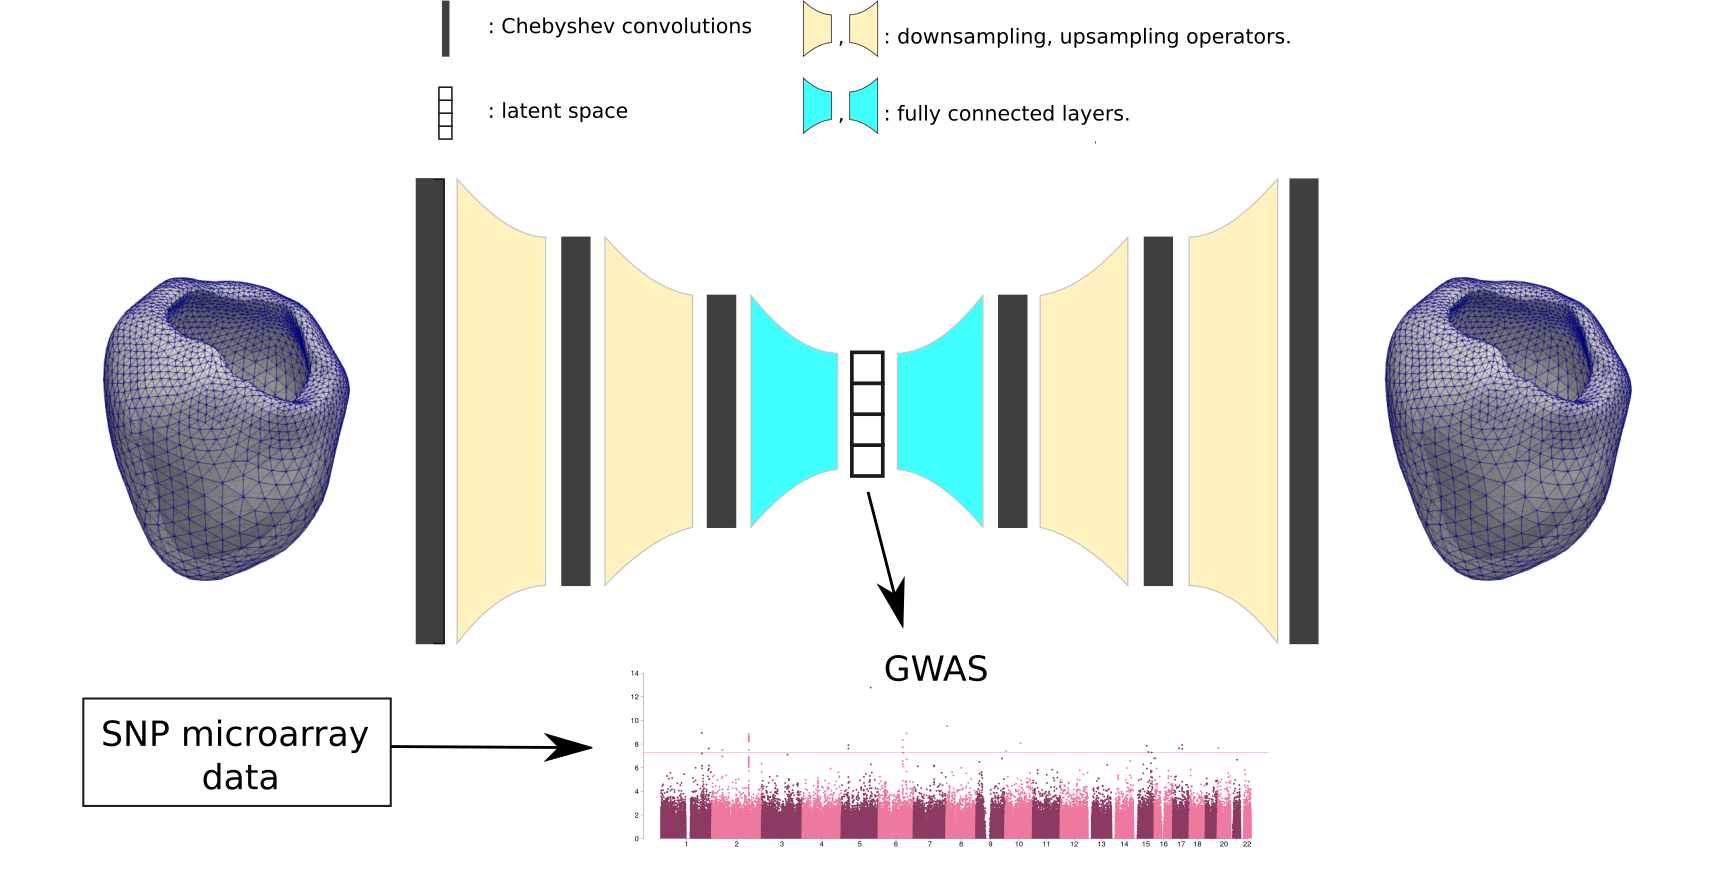
\includegraphics[width=\textwidth]{figs/flowchart.png}
\caption{Flowchart of the steps performed in this work. First, a graph-convolutional autoencoder is trained and applied to our set of LV meshes to produce low-dimensional representations of these shapes. Then, the components of this representation are tested in a GWAS for association with genetic variants.}
\label{fig:flowchart}
\end{figure*}

The unprecedented amount of linked genetic and cardiac imaging data available within the UK Biobank \cite{ref_ukbb} project allows for a different approach: techniques of unsupervised machine learning can be employed to automatically learn a set of features that best describe the morphology of the heart. Atlas-based methods have been proposed to generate 3D meshes representing cardiac anatomy from volumetric images \cite{ref_rahman, ref_zhuang_regis_2O10}. We build on top of these works, leveraging the latest advances in graph-convolutional neural networks (GCNN) \cite{ref_bronstein_geom_DL} to learn low dimensional representations which consider mesh topology. While standard convolutional neural networks operate on domains with an underlying Euclidean or grid-like structure (e.g. images), geometric deep learning generalises convolutions to non-Euclidean domains such as graphs, meshes and manifolds, taking into account their topology and irregular structure. Previous works proposed the use of mesh autoencoders to model the expression space of face surfaces \cite{ref_coma}. Here we show that such models enable learning anatomical variations from cardiac structures, useful to perform genetic association studies.

In this work, we learn compact and non-linear representations of cardiac anatomy in an unsupervised setting via convolutional mesh autoencoders. We hypothesise that the learned features, due to their ability to explain the shape variability across the population, can help identify genetic loci that impact cardiac morphology. We show that such representations can indeed discover novel genetic associations using GWAS, which was not previously possible with traditional handcrafted IDPs such as  volume, mass and function indices. 
